\phantomsection
\definecolor{dkgreen}{rgb}{0,0.6,0}
\definecolor{gray}{rgb}{0.5,0.5,0.5}
\definecolor{mauve}{rgb}{0.58,0,0.82}


\lstset{frame=tb,
language=R,
aboveskip=3mm,
belowskip=3mm,
showstringspaces=false,
columns=flexible,
numbers=none,
inputencoding=utf8/latin1,
keywordstyle=\color{blue},
numberstyle=\tiny\color{gray},
commentstyle=\color{dkgreen},
stringstyle=\color{mauve},
breaklines=true,
breakatwhitespace=true,
tabsize=3
}

\chapter{Stima dei parametri Distribuzione Normale}

\section{Stima puntuale}

Una problematica particolare che riguarda l'inferenza statistica riguarda il voler studiare una popolazione descritta da una variabile aleatoria osservabile $X$ con una funzione di distribuzione nota ma con un parametro $\theta \in \Theta$ non noto (o più parametri)

\subsection{Metodi per la ricerca di stimatori}

Nei metodi di indagine per l'inferenza statistica, a partire da un campione casuale $X_1, X_2, ..., X_n$ di ampiezza $n$ estratto dalla popolazione si cerca di ottenere informazioni sul parametro non noto $\theta$ mediante l'uso di alcune variabili aleatorie, chiamate \textit{stimatori}, che sono funzioni misurabili del campione casuale.

\noindent \textbf{Definizione:} Uno stimatore $\hat{\theta} = t(X_1, X_2, ..., X_n)$ è una funzione misurabile e osservabile del campione casuale $X_1, X_2, ..., X_n$ i cui valori possono essere usati per stimare un parametro non noto $\theta$ della popolazione. I valori $\hat{\theta}$ assunti da tale stimatore sono detti \textit{stime} del parametro non noto $\theta$. Alcune statistiche tipiche sono la media campionaria e la varianza campionaria.

\subsection{Metodo dei momenti}

Per stimare i parametri non noti, viene impiegato il Metodo dei momenti.

\textbf{Definizione:} Si definisce momento campionario r-esimo relativo ai valori osservati ($x_1, x_2, ..., x_n$) del campione casuale il valore

\[M_r(x_1, x_2, ..., x_n) = \frac{1}{n}\sum_{i=1}^n x_i^r \quad (r = 1, 2, ..., k)\]

Dalla definizione il momento campionario r-esimo è la media aritmetica delle potenze r-esime delle n osservazioni effettuate sulla popolazione. Dunque, con $r = 1$, il momento campionario coincide con il calore osservato dalla media campionaria $\Bar{X}$.

Con k parametri da stimare, uguagliamo i primi k momenti della popolazione con i corrispondenti momenti del campione casuale: se i primi k momenti esistono e sono finiti, il metodo dei momenti si riduce alla risoluzione di un sistema di k equazioni:

\[E(X^r) = M_r(x_1, x_2, ..., x_n) \quad (r = 1, 2, ..., k)\]

Le incognite del sistema sono i parametri $\theta, \theta, ..., \theta$ ed essendo una stima di tali incognite vengono indicati con $\hat{\theta}$. Gli stimatori $\hat{\Theta}$ dei parametri non noti, definiti \textit{stimatori del metodo dei momenti}, sono ottenuti al variare dei possibili campioni osservati.

\vspace{5mm}
\noindent \textbf{Popolazione normale}

Con il metodo dei momenti, si è interessati dunque a determinare gli stimatori dei parametri $\mu$ e $\delta^2$ di una popolazione normale di densità di probabilità

\[f_X(x) = \frac{1}{\delta \sqrt{2\pi}} e^{-\frac{(x - \mu)^2}{{2\delta}^2}}, \quad x \in \mathbb{R}, (\mu \in \mathbb{R}, \delta > 0)\]

L'applicazione del metodo dei momenti per la risoluzione del sistema $M_r$ permette di ottenere come stimatore del valore medio $\mu$ la media campionaria $\Bar{X}$ e come stimatore della varianza $\delta^2$ la variabile aleatoria $(n-1)S^2/n$.

\vspace{5mm}
\noindent \textbf{Metodo dei momenti - applicazione dataset}

Applicando il metodo dei momenti al campione in esame descritto da una variabile aleatoria normale, si ottiene: 

\vspace{5mm}
\begin{lstlisting}
  stima_mu <- mean(ds)
  stima_mu
  [1] 1.996316

  stima_s2 <- round((length(ds) - 1) * var(ds) / length(ds), digits = 2)
  stima_s <- sqrt(stima_s2)
  stima_s
  [1] 0.509902
\end{lstlisting}
\vspace{5mm}

La stima del parametro $\mu$ con il metodo dei momenti è $\hat{\mu} = 1.996316$ e la stima del parametro $\delta$ con il metodo dei momenti è $\hat{\delta} = 0.509902$. Come è possibile notare dal codice è stata presa in considerazione la deviazione standard $\delta$ effettuando quindi la radice della varianza.

\subsection{Metodo della massima verosimiglianza}

Il metodo della massima verosimiglianza è il più importante per la stima dei parametri non noti di una popolazione e viene solitamente preferito al metodo dei momenti. Al fine di illustrare questo metodo, occorre introdurre la funzione di verosimiglianza

\noindent \textbf{Definizione:} Sia $X_1, X_2, ..., X_n$ un campione casuale di ampiezza n estratto dalla popolazione. La funzione di verosimiglianza $L(\theta_1, \theta_2, ..., \theta_k) =L(\theta_1, \theta_2, ..., \theta_k ; x_1, x_2, ..., x_n)$ del campione osservato $(x_1, x_2, ..., x_n)$ è la funzione di probabilità congiunta (nel caso di popolazione discreta) oppure la funzione densità di probabilità congiunta (nel caso di popolazione assolutamente continua) del campione casuale $X_1, X_2, ..., X_n$, ossia:

\[L(\theta_1, \theta_2, ..., \theta_k) =L(\theta_1, \theta_2, ..., \theta_k ; x_1, x_2, ..., x_n) \]
\[= f(x_1;\theta_1, \theta_2, ..., \theta_k) f(x_2;\theta_1, \theta_2, ..., \theta_k) ... f(x_n;\theta_1, \theta_2, ..., \theta_k)\]

Il metodo della massima verosimiglianza consiste nella massimizzazione della funzione di verosimiglianza rispetto ai parametri $\theta_1, \theta_2, ..., \theta_k$, cercando di determinare da quale funzione di probabilità congiunta (nel caso di una popolazione discreta) oppure di densità di probabilità congiunta (nel caso di popolazione assolutamente continua) è più verosimile (plausibile) che provenga il campione osservato ($x_1, x_2, ...., x_n$). Pertanto, si cercano di determinare i valori $\theta_1, \theta_2, ..., \theta_k$ che rendono massima la funzione di verosimiglianza, offrendo in un certo senso la migliore spiegazione del campione osservato ($x_1, x_2, ..., x_n$).

I valori di $\theta_1, \theta_2, ..., \theta_k$ che massimizzano la funzione di verosimiglianza sono indicati con $\hat\theta_1, \hat\theta_2, ..., \hat\theta_k$ e costituiscono le stime di massima verosimiglianza dei parametri non noti $\theta_1, \theta_2, ..., \theta_k$ della popolazione. Tali stime dipendono dal campione osservato $(x_1, x_2, ..., x_n)$ e quindi al variare dei possibili campioni osservati si ottengono gli stimatori della massima verosimiglianza $\hat\theta_1, \hat\theta_2, ..., \hat\theta_k$ dei parametri non noti $\theta_1, \theta_2, ..., \theta_k$ della popolazione, detti \textit{stimatori di massima verosimiglianza}.

\vspace{5mm}
\noindent \textbf{Popolazione normale}

Si desidera determinare lo stimatore di massima verosimiglianza dei parametri $\mu$ e $\delta^2$ di una popolazione normale caratterizzata da funzione densità di probabilità

\[f_x(x) = \frac{1}{\sqrt{2\pi \delta^2}} exp\{-\frac{(x - \mu)^2}{2\delta^2}\} \quad (x \in \mathbb{R}, \mu \in \mathbb{R}, \delta > 0)\]

si ha

\[L(\mu, \delta^2) = (\frac{1}{\sqrt{2\pi \delta^2}}^n exp\{-\sum_{i=1}^n \frac{(x_i - \mu)^2}{2\delta^2}\} \quad (\mu \in \mathbb{R}, \delta > 0)\]

dove le $x_i \in \mathbb{R}$. Si nota che

\[log L(\mu, \delta^2) = -\frac{n}{2}log\delta^2 - \frac{n}{2}log(2\pi) - \frac{1}{2\delta^2}\sum_{i=1}^n(x_i - \mu)^2 \quad (\mu \in \mathbb{R}, \delta > 0)\]

e quindi si ha

\[\frac{\theta logL(\mu, \delta^2)}{\theta \mu} = \frac{1}{\delta^2}\sum_{i=1}^n(x_i - \mu) = \frac{n}{\delta^2}(\frac{1}{n}\sum_{i=1}^n x_i - \mu)\]

\[\frac{\theta logL(\mu, \delta^2)}{\theta \delta^2} = -\frac{n}{2\delta^2} + \frac{1}{2\delta^4}\sum_{i=i}^n(x_i - \mu)^2 = -\frac{n}{2\delta^4}(\delta^2 - \frac{1}{n} \sum_{i=i}^n (x_i - \mu)^2)\]

Le stime di massima verosimiglianza dei parametri $\mu$ e $\delta^2$ sono rispettivamente

\[\hat{\mu} = \frac{1}{n}\sum_{i=1}^n x_i, \quad \hat{\delta^2} = \frac{1}{n}\sum_{i=1}^n (x_i - \hat{\mu})^2\]

Lo stimatore di massima verosimiglianza e dei momenti del valore medio $\mu$ è la media campionaria $\Bar{X}$; invece, lo stimatore di massima verosimiglianza e dei momenti della varianza $\delta^2$ è $(n-1)S^2/n$.

\subsection{Disuguaglianza di Cramèr-Rao}

Sia $\hat{\Theta} = t(X_1, X_2, ..., X_n)$ uno stimatore corretto del parametro non noto $\theta$ di una popolazione caratterizzata da funzione di probabilità (nel caso discreto) oppure densità di probabilità (nel caso assolutamente continuo) $f(x;\theta)$. Se sono soddisfatte le ipotesi seguenti

\begin{enumerate}
    \item $\frac{\theta}{\theta \omega} log f(x;\omega) \quad$ esiste per ogni x e per ogni $\alpha \in \Theta,$
    \item $E\{[\frac{\theta}{\theta \omega} log f(X;\omega)]^2\} \quad$ esiste finito per ogni $\alpha \in \Theta$
\end{enumerate}

la varianza dello stimatore $\hat{\Theta}$ soddisfa la disuguaglianza

\[Var(\hat{\Theta}) \geq \frac{1}{nE\{[\frac{\theta}{\theta \omega} log f(X;\omega)]^2\}}\]

Si noti che la disuguaglianza di Cramèr-Rao individua l'estremo inferiore della varianza di uno stimatore corretto, ma non implica che esista sempre uno stimatore con varianza uguale al suo estremo.

Se 

\[Var(\hat{\Theta}) = \frac{1}{nE\{[\frac{\theta}{\theta \omega} log f(X;\omega)]^2\}}\]

allora $\hat{\Theta}$ è uno stimatore corretto con varianza uniformemente minima per il parametro $\theta$

\vspace{5mm}
\noindent \textbf{Popolazione normale}

Si desidera verificare che $\Bar{X}$ è uno stimatore corretto con varianza uniformemente minima del valore medio $E(X) = \mu$ di una popolazione normale descritta da una variabile aleatoria $X ~ N (\mu, \delta)$ avente varianza nota $\delta^2$. Tale stimatore è stato precedentemente determinato sia con il metodo dei momenti che con il metodo della massima verosimiglianza. La densità di probabilità che caratterizza la popolazione è:

\[f_X(x) = \frac{1}{\delta \sqrt{2\pi}} exp\{-\frac{(x - \mu)^2}{2\delta^2}\}, \quad x \in \mathbb{R} \quad (\mu \in \mathbb{R}, \delta > 0)\]

Poiché $E(X) = \mu$, il parametro da stimare è $\theta = \mu$. Osserviamo che

\[log f(x;\mu) = -log(\delta \sqrt{2\pi}) - \frac{(x - \mu)^2}{2\delta^2}\]

e quindi

\[\frac{\theta}{\theta \mu} log f(x;\mu) = \frac{x - \mu}{\delta^2}\]

Essendo $Var(X) = \delta^2$ risulta

\[E\{[\frac{\theta}{\theta \mu} log f(X;\mu)]^2\} = E[(\frac{X-\mu}{\delta^2})^2] = \frac{1}{\delta^4}E[(X - \mu)^2] = \frac{Var(X)}{\delta^4} = \frac{1}{\delta^2}\]

e quindi

\[Var(\Bar{X}) = \frac{\delta^2}{n}, \quad \frac{1}{nE\{[\frac{\theta}{\theta \mu} log f(X;\mu)]^2\}} = \frac{\delta^2}{n}\]

Segue quindi che $\Bar{X}$ è uno stimatore corretto con varianza uniformemente minima del valore medio $\mu$ di una popolazione normale con varianza nota $\delta^2$.

\subsection{Stimatore Asintoticamente Corretto}

Uno stimatore $\hat{\Theta_n} = t(X_1, X_2, ..., X_n)$ del parametro non noto $\theta$ della popolazione è detto asintoticamente corretto (asintoticamente non distorto) se e solo se per ogni $\theta \in \Theta$ si ha

\[\lim_{n\to\infty} E(\hat{\Theta_n}) = \theta,\]

ossia se il valore medio dello stimatore $\Theta_n$ tende al crescere dell'ampiezza del campione casuale al corrispondente parametro non noto della popolazione

\noindent \textbf{Stimatore asintoticamente corretto della varianza di una popolazione}

Si desidera verificare che 

\[\hat{\Theta_n} = \frac{n-1}{n}S^2 = \frac{1}{n} \sum_{i=1}^n(X_i - \Bar{X})^2\]

è uno stimatore asintoticamente corretto della varianza $\delta^2$ di una popolazione.

Ricordando che $E(S^2) = \delta^2$, si ottiene immediatamente:

\[\lim_{n\to\infty} E(\hat{\Theta_n}) = [\lim_{n\to\infty} \frac{n-1}{n} E(S^2)=\delta^2\]

In particolare, per una popolazione normale lo stimatore $(n-1)S^2/n$ della varianza $\delta^2$, individuato sia con il metodo dei momenti che con il metodo della massima verosimiglianza, è asintoticamente corretto. 

\begin{figure}[!htbp]
    \centering
    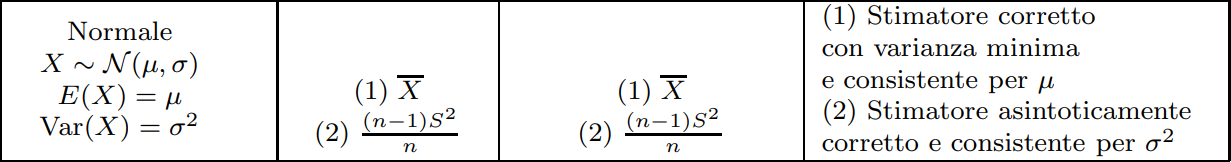
\includegraphics[height=2.2cm]{capitoli/images/2_stima_parametri/tabella.png}
\end{figure}
\vspace{5mm}

\section{Intervalli di confidenza}

Alla stima puntuale di un parametro non noto di una popolazione (costituita da un singolo valore reale) spesso si preferisce sostituire un intervallo di valori, detto \textbf{intervallo di confidenza} (o intervallo di fiducia), ossia si cerca di determinare in base ai dati del campione due limiti (uno inferiore e uno superiore) entro i quali sia compreso il parametro non noto con un certo \textbf{coefficiente di confidenza} (detto anche grado di fiducia).

\noindent \textbf{Definizione:} Fissato un coefficiente di confidenza $1-\alpha (0 < \alpha < 1)$, se è possibile scegliere le statistiche $\underline{C_n}$ e $\Bar{C_n}$ in modo tale che

\[P(\underline{C_n} < \theta < \Bar{C_n}) = 1 - \alpha\],

allora si dice che $(\underline{C_n}, \Bar{C_n})$ è un intervallo di confidenza di grado $1 - \alpha$ per $\theta$. Inoltre, le statistiche $\underline{C_n = g_1 = (X_1, X_2, ..., X_n)}$ e $\Bar{C_n} = g_2 = (X_1, X_2, ..., X_n)$ sono dette limite inferiore e superiore dell'intervallo di confidenza.

Se $g_1(x)$ e $g_2(x)$ sono i valori assunti dalle statistiche $\underline{C_n}$ e $\Bar{C_n}$ per il campione osservato $x = (x_1, x_2, ..., x_n)$, allora l'intervallo $(g_1(x), g_2(x))$ è detto stima dell'intervallo di confidenza di grado $1-\alpha$ per $\theta$ e i punti finali $g_1(x)$ e $g_2(x)$ di tale intervallo sono detti rispettivamente stima del limite inferiore e stima del limite superiore dell'intervallo di confidenza. La scelta dell'intervallo di confidenza deve essere effettuata in base ad alcune proprietà statistiche. Ad esempio, fissato un coefficiente di confidenza $1-\alpha$, alcune proprietà desiderabili sono che la lunghezza dell'intervallo di confidenza 

\[L(X_1, X_2, ..., X_n;1-\alpha) = \underline{C_n} - \Bar{C_n}\]

sia la più piccola possibile oppure che la lunghezza media di tale intervallo sia la più piccola possibile.

\subsection{Metodo Pivotale}

Un metodo per la costruzione degli intervalli di confidenza è il metodo pivotale. Tale metodo consiste essenzialmente nel determinare una variabile aleatoria di pivot $\gamma(X_1, X_2, ..., X_n;\theta)$ che dipende dal campione casuale $X_1, X_2, ..., X_n$ e dal parametro non noto $\theta$ e la cui funzione di distribuzione non contiene il parametro da stimare. Tale variabile aleatoria non è una statistica poiché dipende dal parametro non noto $\theta$ e quindi non è osservabile.

Sia $X_1, X_2, ..., X_n$ un campione casuale di ampiezza n estratto da una popolazione normale con valore medio $\mu$ e varianza $\delta^2$ si possono analizzare i seguenti problemi:

\begin{enumerate}
    \item determinare un intervallo di confidenza di grado $1 - \alpha$ per il valore medio $\mu$ nel caso in cui la varianza di $\delta^2$ della popolazione normale è nota;
    \item determinare un intervallo di confidenza di grado $1 - \alpha$ per il valore medio $\mu$ nel caso in cui la varianza della popolazione normale è non nota;
    \item determinare un intervallo di confidenza di grado $1 - \alpha$ per la varianza $\delta^2$ nel caso in cui il valore medio $\mu$ della popolazione normale è noto;
    \item determinare un intervallo di confidenza di grado $1 - \alpha$ per la varianza $\delta^2$ nel caso in cui il valore medio della popolazione normale è non noto.
\end{enumerate}

In questo lavoro ci focalizzeremo sul secondo e sul quarto problema.

\vspace{5mm}
\noindent \textbf{Intervallo di confidenza per $\mu$ con varianza non nota}

Per determinare un intervallo di confidenza di grado $1-\alpha$ per il valore medio $\mu$ nel caso in cui la varianza $\delta^2$ della popolazione normale non è nota, utilizziamo il metodo pivotale e consideriamo la variabile aleatoria di pivot:

\[T_n = \frac{\Bar{X_n} - \mu}{S_n/\sqrt{n}}\]

Tale variabile aleatoria dipende dal campione casuale e dal parametro non noto $\mu$. Inoltre, poiché:

\[T_n = \frac{\Bar{X} - \mu}{\delta / \sqrt{n}}\sqrt{\frac{\delta^2}{S_n^2}} = \frac{Z_n}{\sqrt{Q_n}/(n-1)}\]

si ha che $T_n$ è distribuita con legge di Student con $n-1$ gradi di libertà.

Scegliendo nel metodo pivotale $\alpha1 = -t_{\alpha/2,n-1}$ e $\alpha2 = t_{\alpha/2,n-1}$ dove $t_{\alpha/2,n-1}$ è tale che 

\[P(T_n < -t_{\alpha/2,n-1}) = P(T_n>t_{\alpha/2,n-1}) = \frac{\alpha}{2}\]

ne deriva che:

\[P(-t_{\alpha/2,n-1} < T_n < t_{\alpha/2,n-1}) = 1-\alpha\]

Dalla probabilità ottenuta si ottiene:

\[P(\Bar{X}_n - t_{\alpha/2,n-1} \frac{S_n}{\sqrt{n}} <\mu < \Bar{X}_n + t_{\alpha/2,n-1}\frac{S_n}{\sqrt{n}} = 1- \alpha\]

Se poniamo:

\[\underline{C_n} = \Bar{X}_n - t_{\alpha/2,n-1}\frac{S_n}{\sqrt{n}}, \Bar{C}_n = \Bar{X}_n + t_{\alpha/2,n-1}\frac{S_n}{\sqrt{n}}\]

si ha che $(\underline{C_n}, \Bar{C}_n)$ è un intervallo di confidenza di grado $1 - \alpha$ per $\mu$, dove le statistiche $(\underline{C_n}$ e $\Bar{C}_n)$ rappresentano il limite inferiore e superiore rispettivamente. Si può ora definire la lunghezza dell'intervallo di confidenza:

\[L(X_1, X_2, ..., X_n;1-\alpha) = \Bar{C}_n - \underline{C_n} = 2t_{\alpha/2,n-1}\frac{S_n}{\sqrt{n}}\]

Quindi, per ogni fissato campione osservato $(x_1, x_2, ..., x_n)$ a valori sempre più piccoli di $\alpha$, corrispondono lunghezze di intervalli di confidenza sempre più ampi. Da tutto ciò ne deriva che dato un campione $(x_1, x_2, ..., x_n)$ di ampiezza n estratto da una popolazione normale con varianza non nota si ha che la stima dell'intervallo di confidenza di grado $1-\alpha$ per il valore medio $\mu$ è 

\[\Bar{x}_n = t_{\alpha/2,n-1}\frac{S_n}{\sqrt{n}} < \mu < \Bar{x}_n + t_{\alpha/2,n-1}\frac{S_n}{\sqrt{n}}\]

dove $x_n$ e $S_n$ denotano rispettivamente la media e la deviazione standard campionaria delle n osservazioni.

\vspace{5mm}
\noindent \textbf{Metodo pivotale - applicazione}

Si considerino 2 casi in particolare:

\begin{itemize}
    \item $\alpha = 0.05$
    \item $\alpha = 0.01$
\end{itemize}

\vspace{5mm}
\noindent \textbf{Stima dell'intervallo di confidenza di grado $1 - \alpha = 0.95$}

\begin{lstlisting}
  alpha <- 1 - 0.95
  n <- length(ds)
  mean(ds)
  [1] 1.996316
  sd(ds)
  [1] 0.51082
  mean(ds) - qt(1 - alpha / 2, df = n - 1) * sd(ds) / sqrt(n)
  [1] 1.882638
  mean(ds) + qt(1 - alpha / 2, df = n - 1) * sd(ds) / sqrt(n)
  [1] 2.109993
\end{lstlisting}

La stima dell'intervallo di confidenza di grado $1-\alpha = 0.95$ per il quantitativo medio è (1.88, 2.11), ed è osservabile come $\mu$ sia compreso nell'intervallo.

\vspace{5mm}
\noindent \textbf{Stima dell'intervallo di confidenza di grado $1 - \alpha = 0.99$}

\begin{lstlisting}
  alpha <- 1 - 0.99
  n <- length(ds)
  mean(ds)
  [1] 1.996316
  sd(ds)
  [1] 0.51082
  mean(ds) - qt(1 - alpha / 2, df = n - 1) * sd(ds) / sqrt(n)
  [1] 1.84557
  mean(ds) + qt(1 - alpha / 2, df = n - 1) * sd(ds) / sqrt(n)
  [1] 2.147062
\end{lstlisting}

La stima dell'intervallo di confidenza di grado $1-\alpha = 0.5$ per il quantitativo medio è (1.85, 2.15), ed è osservabile come $\mu$ sia compreso nell'intervallo.

Si nota che aumentando il grado di fiducia, aumenta anche la lunghezza dell'intervallo di confidenza.

\vspace{5mm}
\noindent \textbf{Intervallo di confidenza per $\delta^2$ con valore medio non noto}

Per determinare un intervallo di confidenza di grado $1-\alpha$ per la varianza $\delta^2$ nel caso in cui il valore medio $\mu$ della popolazione non è noto, utilizziamo il metodo pivotale e consideriamo la variabile aleatoria di pivot:

\[Q_n = \frac{(n-1)S_n^2}{\delta^2} = \frac{1}{\delta^2}\sum_{i=1}^n(X_i - \Bar{X}_n)^2\]

Tale variabile aleatoria dipende dal campione casuale e dal parametro non noto $\delta^2$ ed è distribuita con legge chi-quadrato con n-1 gradi di libertà.

Scegliendo nel metodo pivotale $\alpha_1 = X^2_{1-\alpha/2,n-1}$ e $\alpha_2 = X^2_{\alpha/2,n-1}$ ina maniera tale che

\[P(0<Q_n<X^2_{1-\alpha/2,n-1} = P(Q_n>X^2_{\alpha/2,n-1} = \frac{\alpha}{2}\]

ne deriva che:

\[P(X^2_{1-\alpha/2,n-1} < Q_n < X^2_{\alpha/2,n-1}) = 1-\alpha\]

Dalla probabilità ottenuta abbiamo:

\[P(X^2_{1-\alpha/2,n-1} < \frac{(n-1)S_n^2}{\delta^2}<X^2_{\alpha/2,n-1} = 1-\alpha\]

che è equivalente a richiedere che 

\[P(\frac{(n-1)S_n^2}{X^2_{\alpha/2,n-1}} < \delta^2 < \frac{(n-1)S^2_n}{X^2_{1-\alpha/2,n-1}}) = 1-\alpha\]

Se poniamo

\[\underline{C_n} = \frac{(n-1)S_n^2}{X^2_{\alpha/2,n-1}}, \quad \Bar{X}_n = \frac{(n-1)S^2_n}{X^2_{1-\alpha/2,n-1}}\]

si ha che $(\underline{C_n}, \Bar{C}_n)$ è un intervallo di confidenza di grado $1-\alpha$ per $\delta^2$, dove le statistiche $\underline{C_n}$ e $\Bar{C}_n$ rappresentano il limite inferiore e superiore rispettivamente. Quindi, per ogni fissato campione osservato $(x_1, x_2, ..., x_n)$, a valori sempre più piccoli di $\alpha$ corrispondono lunghezze di intervalli di confidenza sempre più ampi. Da tutto ciò ne deriva che, dato un campione $(x_1, x_2, ..., x_n)$ di ampiezza n estratto da una popolazione normale con valore medio non noto si ha che la stima dell'intervallo di confidenza di grado $1-\alpha$ per la  varianza $\delta^2$ è

\[\frac{(n-1)S_n^2}{X^2_{\alpha/2,n-1}} < \delta^2 < \frac{(n-1)S^2_n}{X^2_{1-\alpha/2,n-1}}\]

dove

\[s_n^2 = \frac{1}{n-1} \sum_{i+1}^n (x_i - \Bar{x})n)^2\]

denota la varianza campionaria delle n osservazioni.

\vspace{5mm}
\noindent \textbf{Metodo pivotale - applicazione}

Si considerino 2 casi in particolare:

\begin{itemize}
    \item $\alpha = 0.05$
    \item $\alpha = 0.01$
\end{itemize}

\vspace{5mm}
\noindent \textbf{Stima dell'intervallo di confidenza di grado $1 - \alpha = 0.95$}

\begin{lstlisting}
 alpha <- 1 - 0.95
 n <- length(ds)
 var(ds)
 [1] 0.2609371
 (n-1)*var(ds)/qchisq(1-alpha/2,df=n-1)
 [1] 0.1954441
 (n-1)*var(ds)/qchisq(alpha/2,df=n-1)
 [1] 0.3660883
\end{lstlisting}

La stima dell'intervallo di confidenza di grado $1-\alpha = 0.5$ per la varianza è (0.195, 0.366) ed è osservabile come $\delta^2$ sia compreso in questo intervallo.

\vspace{5mm}
\noindent \textbf{Stima dell'intervallo di confidenza di grado $1 - \alpha = 0.99$}

\vspace{5mm}
\begin{lstlisting}
 alpha <- 1 - 0.99
 n <- length(ds)
 var(ds)
 [1] 0.2609371
 (n-1)*var(ds)/qchisq(1-alpha/2,df=n-1)
 [1] 0.1790709
 (n-1)*var(ds)/qchisq(alpha/2,df=n-1)
 [1] 0.4092025
\end{lstlisting}

La stima dell'intervallo di confidenza di grado $1-\alpha = 0.5$ per la varianza è (0.179, 0.409) ed è osservabile come $\delta^2$ sia compreso in questo intervallo.

Si nota che aumentando il grado di fiducia, aumenta la lunghezza dell'intervallo di confidenza.

Per una popolazione normale, le stime per intervallo del valore $\mu$ e della varianza $\delta^2$ della popolazione possono essere effettuate qualsiasi sia la dimensione del campione casuale osservato. Ciò dipende dalla circostanza favorevole di conoscere la distribuzione esatta della variabile pivotale considerata: normale e di Student per la stima del valore medio e chi-quadrato per la stima della varianza.
%################################################

\newpage